\documentclass[a4paper]{article}
\usepackage[a4paper,margin=0mm]{geometry}
\usepackage{fontspec}
\usepackage{unicode-math}
\usepackage{tikz}
\usetikzlibrary{calc}
\usepackage[table]{xcolor}
\usepackage[absolute]{textpos}
\usepackage{enumitem}
\usepackage{array}
\usepackage{multirow}

\setmainfont{Libertinus Serif}
\setsansfont{Libertinus Sans}
\setmathfont{Libertinus Math}

\definecolor{accent}{HTML}{0F6A52}
\definecolor{badge}{HTML}{A9CFC2}
\definecolor{ink}{HTML}{2A2E30}

\setlength{\TPHorizModule}{1mm}
\setlength{\TPVertModule}{1mm}
\setlength{\parindent}{0pt}
\pagestyle{empty}
\binoppenalty=10000 \relpenalty=10000

\newcommand{\LCOL}{16mm}
\newcommand{\RCOL}{111mm}
\newcommand{\COLW}{83mm}

\newcommand{\topicheader}[2]{%
\begin{textblock*}{194mm}(16mm,10mm)
\begin{tikzpicture}
\node[fill=accent,text=white,font=\sffamily\bfseries\fontsize{13}{13}\selectfont,
      minimum width=9mm,minimum height=9mm,inner sep=0pt] at (4.5mm,-4.5mm) {#1};
\node[font=\sffamily\bfseries\fontsize{15}{16}\selectfont,text=ink,anchor=west] at (12mm,-4.5mm) {#2};
\end{tikzpicture}
\end{textblock*}
\begin{textblock*}{194mm}(16mm,22.5mm)

\begin{tikzpicture}
\fill[accent] (0,0) rectangle (194mm,0.5mm);
\end{tikzpicture}
\end{textblock*}
}

\newcommand{\pagefooter}[1]{%
\begin{textblock*}{194mm}(8mm,286.41mm)
  
\begin{tikzpicture}
    \fill[accent] (0,0) rectangle (194mm,0.6mm);
  \end{tikzpicture}
\end{textblock*}
\begin{textblock*}{63.59mm}(8mm,288.27mm)
  {\sffamily\bfseries\color{accent}\fontsize{13}{16}\selectfont SAT 1200+}
\end{textblock*}
\begin{textblock*}{10mm}(188mm,288.27mm)
  \centering{\sffamily\color{accent}\fontsize{14}{16}\selectfont #1}
\end{textblock*}
}

\newcommand{\colrule}[2]{%
\begin{textblock*}{1mm}(105mm,#1mm)
\begin{tikzpicture}
\draw[black!65,line width=0.5pt] (0,0) -- (0,#2mm);
\end{tikzpicture}
\end{textblock*}
}

% Page kicker: left = module line, right = question range
\newcommand{\pagekicker}[2]{%
\begin{textblock*}{194mm}(16mm,25.2mm)
{\sffamily\bfseries\fontsize{10.5}{12}\selectfont\color{accent}#1}\hfill{\sffamily\fontsize{10}{12}\selectfont\color{black!70}#2}
\end{textblock*}
}

\setlength{\fboxsep}{1.4pt}
\setlength{\fboxrule}{0.5pt}
\newcommand{\pnum}[1]{\fcolorbox{ink}{white}{\sffamily\bfseries\fontsize{8}{8}\selectfont #1}~}

% centered display line inside a stem
\newcommand{\dsp}[1]{\par\vspace{1.4mm}\centerline{#1}\vspace{1.8mm}}

% student-produced response box
\newcommand{\gridbox}{%
\par\vspace{3mm}\noindent

\begin{tikzpicture}
\node[anchor=south west,font=\sffamily\bfseries\fontsize{7.5}{9}\selectfont,text=accent,inner sep=0pt] at (0,0.3mm) {STUDENT-PRODUCED RESPONSE};
\draw[ink,line width=0.7pt] (0,-9.5mm) rectangle (40mm,-0.8mm);
\node[anchor=west,font=\sffamily\fontsize{7.5}{9}\selectfont,text=black!55,inner sep=0pt] at (43mm,-5.2mm) {Write your answer in the box.};
\end{tikzpicture}\par}

\arrayrulecolor{accent}
\setlength{\arrayrulewidth}{0.7pt}
\renewcommand{\arraystretch}{1.35}

\newcommand{\figwrap}[1]{\par\vspace{2.5mm}\centerline{{\arrayrulecolor{ink}\setlength{\arrayrulewidth}{0.5pt}\renewcommand{\arraystretch}{1.3}#1}}\vspace{0.5mm}}

\begin{document}

% ================= PAGE 1: Mock Test 1 -- instructions + geometry reference sheet =================
\topicheader{1}{Mock Test 1}
\pagefooter{1}
\mbox{}%

\newcommand{\cardhead}[1]{{\sffamily\bfseries\color{accent}\fontsize{11.5}{14}\selectfont #1}\par\vspace{0.6mm}%
{\color{accent}\rule{\linewidth}{0.5pt}}\par\vspace{1.6mm}}
\newcommand{\bul}{\item[\textcolor{accent}{\rule[0.2mm]{1.5mm}{1.5mm}}]}

\begin{textblock*}{194mm}(16mm,28mm)
{\sffamily\bfseries\color{accent}\fontsize{26}{28}\selectfont Mock Test 1\par}
\vspace{1mm}
{\sffamily\color{ink}\fontsize{11}{14}\selectfont Full-length digital SAT Math practice \;\textperiodcentered\; 2 modules $\times$ 22 questions $\times$ 35 minutes\par}
\end{textblock*}

\begin{textblock*}{\COLW}(\LCOL,53mm)
{\fontsize{9.4}{12.2}\selectfont
\cardhead{How this test works}
\renewcommand{\arraystretch}{1.3}\setlength{\tabcolsep}{4pt}
\noindent\begin{tabular}{|>{\raggedright\arraybackslash}p{20mm}|>{\centering\arraybackslash}p{15mm}|>{\centering\arraybackslash}p{13mm}|>{\centering\arraybackslash}p{19mm}|}
\hline
\rowcolor{badge!55}\textbf{Module} & \textbf{Questions} & \textbf{Time} & \textbf{Calculator}\\\hline
Module 1 & 22 & 35 min & allowed\\\hline
Module 2 & 22 & 35 min & allowed\\\hline
\end{tabular}\par\vspace{2.2mm}
\begin{itemize}[leftmargin=5mm,itemsep=1.2mm,topsep=0mm,parsep=0mm]
\bul Time each module separately: 35 minutes, not a minute more. Rest for 5--10 minutes between the two modules.
\bul Use a calculator (the built-in Desmos graphing calculator or any approved calculator) on both modules.
\bul Module 1 is a standard mix of easy, medium and hard questions. Module 2 is the \emph{harder route} you reach by doing well on Module 1.
\bul Answer every question. There is no penalty for a wrong answer.
\bul Unless a problem says otherwise, all numbers are real, a function's domain is every real number for which it is defined, and figures are not necessarily drawn to scale.
\bul Do not look at any answers while you work. When you finish both modules, score yourself with the \textbf{Answer Sheets} section at the end of this book.
\end{itemize}
}
\end{textblock*}

\begin{textblock*}{\COLW}(\RCOL,53mm)
{\fontsize{9.4}{12.2}\selectfont
\cardhead{Student-produced responses (grid-ins)}
Some questions have no answer choices. Work out the answer and write it in the answer box (on the real test you type it in).
\begin{itemize}[leftmargin=5mm,itemsep=1.2mm,topsep=1.6mm,parsep=0mm]
\bul You may give an integer, a decimal, or a fraction. For one answer, $9/2$ and $4.5$ are both correct.
\bul Never enter a mixed number: write $7/2$ or $3.5$, not $3\,1/2$ (it would be read as $31/2$).
\bul Do not enter symbols or units such as \$, \%, or $\pi$. Enter the number only.
\bul An answer may use at most 5 characters (6 if it is negative), counting the slash and the decimal point.
\bul If an answer is a repeating decimal, enter it as a fraction such as $2/3$, or fill all the digits that fit: $0.6666$ or $0.6667$.
\bul If you find more than one correct answer, enter only one of them.
\end{itemize}
\vspace{1.2mm}
\noindent\fcolorbox{accent}{badge!25}{\parbox{\dimexpr\linewidth-2\fboxsep-2\fboxrule}{\centering\sffamily\fontsize{8.5}{11}\selectfont
\textbf{Example.} Answer $4\tfrac12$ \;$\rightarrow$\; enter \textbf{9/2} or \textbf{4.5}\par}}
}
\end{textblock*}

% ---- Geometry reference sheet (full width card) ----
\begin{textblock*}{178mm}(16mm,156mm)
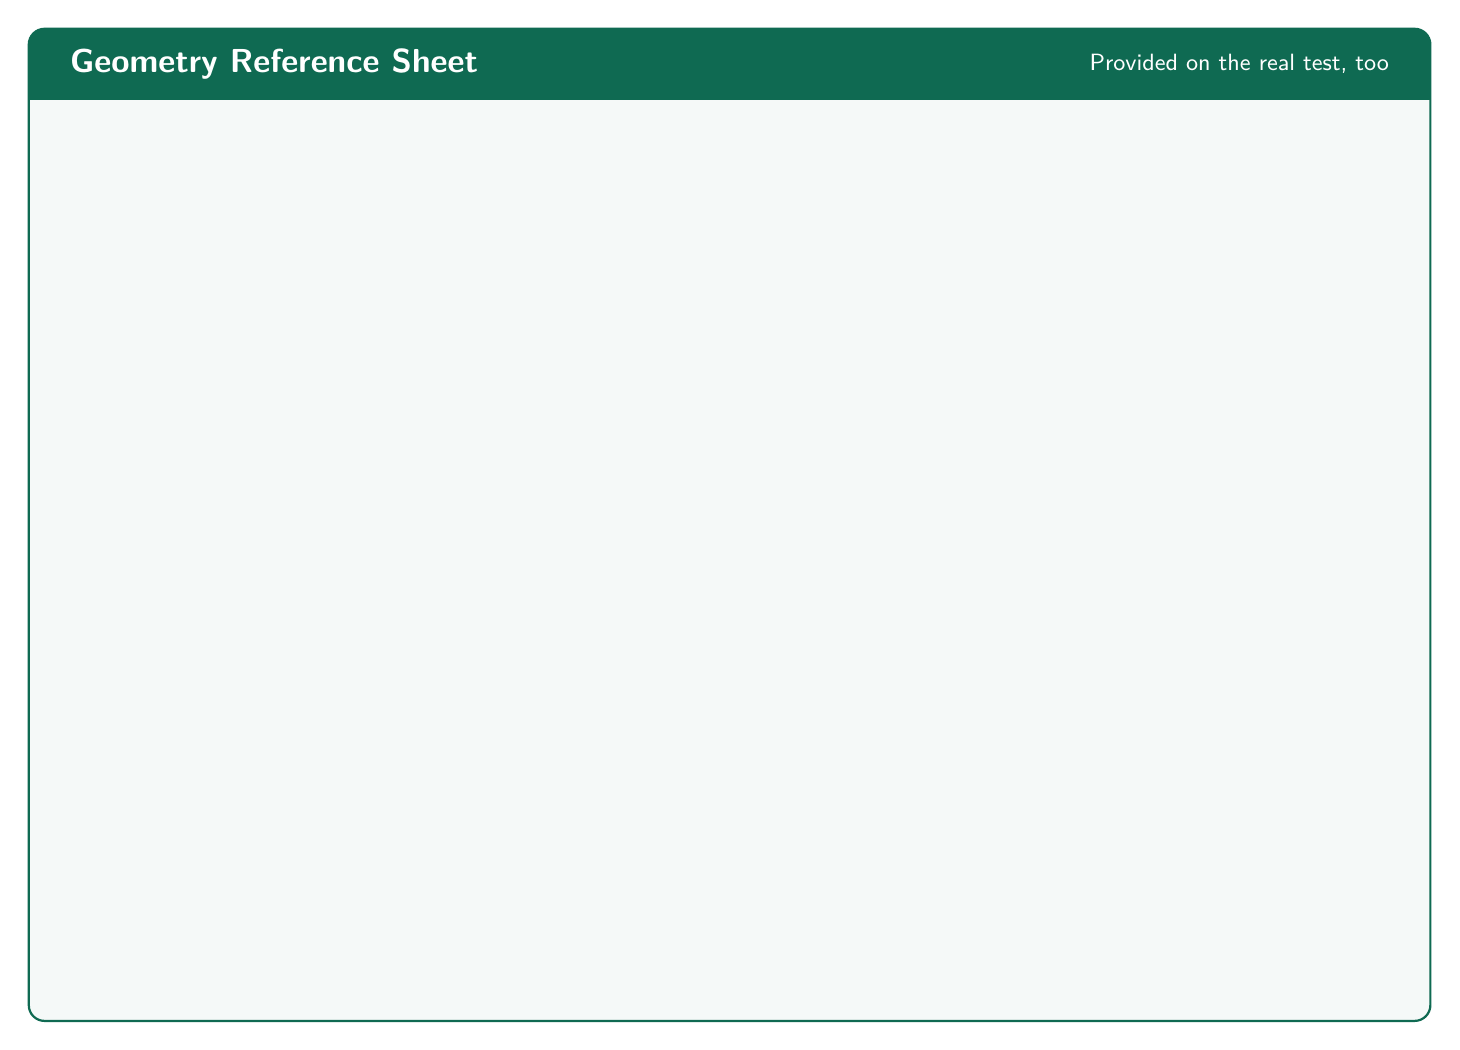
\begin{tikzpicture}
\draw[accent,line width=0.8pt,rounded corners=2mm,fill=badge!12] (0,0) rectangle (178mm,-126mm);
\fill[accent,rounded corners=2mm] (0,0) rectangle (178mm,-9mm);
\fill[accent] (0,-5mm) rectangle (178mm,-9mm);
\node[anchor=west,text=white,font=\sffamily\bfseries\fontsize{12}{14}\selectfont] at (4mm,-4.5mm) {Geometry Reference Sheet};
\node[anchor=east,text=white,font=\sffamily\fontsize{8.5}{10}\selectfont] at (174mm,-4.5mm) {Provided on the real test, too};
\end{tikzpicture}
\end{textblock*}

\newcommand{\refcell}[3]{\begin{textblock*}{42mm}(#1mm,#2mm)\begin{minipage}[t][36mm][t]{42mm}\centering #3\end{minipage}\end{textblock*}}
\newcommand{\refin}[2]{\parbox[b][26mm][b]{42mm}{\centering #1}\par\vspace{1.6mm}{\fontsize{9.6}{11.5}\selectfont #2}}
\tikzset{rf/.style={ink,line width=0.65pt},lb/.style={font=\fontsize{8.5}{9.5}\selectfont,inner sep=1.2pt}}

% ---------- row 1
\refcell{18}{167}{\refin{\begin{tikzpicture}[scale=1.25]
\draw[rf] (0,0) circle (9mm); \draw[rf] (0,0)--(9mm,0); \fill[ink] (0,0) circle (0.7pt);
\node[lb,above] at (4.5mm,0) {$r$};
\end{tikzpicture}}{Circle\\$A=\pi r^{2}$,\; $C=2\pi r$}}
\refcell{62}{167}{\refin{\begin{tikzpicture}[scale=1.25]
\draw[rf] (0,0) rectangle (22mm,12mm);
\node[lb,below] at (11mm,0) {$\ell$}; \node[lb,right] at (22mm,6mm) {$w$};
\end{tikzpicture}}{Rectangle\\$A=\ell w$}}
\refcell{106}{167}{\refin{\begin{tikzpicture}[scale=1.25]
\draw[rf] (0,0)--(22mm,0)--(7mm,13mm)--cycle;
\draw[rf,dashed] (7mm,0)--(7mm,13mm);
\draw[rf] (7mm,0)++(0,1.8mm)--++(1.8mm,0)--++(0,-1.8mm);
\node[lb,below] at (11mm,0) {$b$}; \node[lb,left] at (7mm,6.5mm) {$h$};
\end{tikzpicture}}{Triangle\\$A=\tfrac12 bh$}}
\refcell{150}{167}{\refin{\begin{tikzpicture}[scale=1.25]
\draw[rf] (0,0)--(18mm,0)--(0,12mm)--cycle;
\draw[rf] (0,1.8mm)--(1.8mm,1.8mm)--(1.8mm,0);
\node[lb,below] at (9mm,0) {$a$}; \node[lb,left] at (0,6mm) {$b$}; \node[lb,above right] at (9mm,6mm) {$c$};
\end{tikzpicture}}{Right triangle\\$c^{2}=a^{2}+b^{2}$}}

% ---------- row 2
\refcell{18}{204}{\refin{\begin{tikzpicture}[scale=1.25]
\draw[rf] (0,0)--(19.053mm,0)--(0,11mm)--cycle;
\draw[rf] (0,1.8mm)--(1.8mm,1.8mm)--(1.8mm,0);
\node[lb,below] at (9.5mm,0) {$x\sqrt3$}; \node[lb,left] at (0,5.5mm) {$x$}; \node[lb,above right] at (9.5mm,5.5mm) {$2x$};
\node[lb] at (14.6mm,1.9mm) {\fontsize{6.5}{7}\selectfont$30^\circ$}; \node[lb] at (3.2mm,8.2mm) {\fontsize{6.5}{7}\selectfont$60^\circ$};
\end{tikzpicture}}{$30^\circ$--$60^\circ$--$90^\circ$ triangle}}
\refcell{62}{204}{\refin{\begin{tikzpicture}[scale=1.25]
\draw[rf] (0,0)--(10mm,0)--(0,10mm)--cycle;
\draw[rf] (0,1.8mm)--(1.8mm,1.8mm)--(1.8mm,0);
\node[lb,below] at (5mm,0) {$s$}; \node[lb,left] at (0,5mm) {$s$}; \node[lb,above right] at (5mm,5mm) {$s\sqrt2$};
\end{tikzpicture}}{$45^\circ$--$45^\circ$--$90^\circ$ triangle}}
\refcell{106}{204}{\refin{\begin{tikzpicture}[scale=1.2]
\draw[rf] (0,0) rectangle (16mm,9mm);
\draw[rf] (16mm,9mm)--(22mm,13mm)--(6mm,13mm)--(0,9mm);
\draw[rf] (16mm,0)--(22mm,4mm)--(22mm,13mm);
\draw[rf,dashed] (6mm,13mm)--(6mm,4mm)--(22mm,4mm); \draw[rf,dashed] (0,0)--(6mm,4mm);
\node[lb,below] at (8mm,0) {$\ell$}; \node[lb,right] at (22mm,8.5mm) {$h$}; \node[lb,below right] at (19mm,2mm) {$w$};
\end{tikzpicture}}{Rectangular solid\\$V=\ell wh$}}
\refcell{150}{204}{\refin{\begin{tikzpicture}[scale=1.2]
\draw[rf] (0,2.2mm) ellipse (7mm and 2.2mm);
\draw[rf] (-7mm,2.2mm)--(-7mm,14mm); \draw[rf] (7mm,2.2mm)--(7mm,14mm);
\draw[rf] (0,14mm) ellipse (7mm and 2.2mm);
\draw[rf,dashed] (0,14mm)--(7mm,14mm); \fill[ink] (0,14mm) circle (0.6pt);
\node[lb,above] at (3.5mm,14mm) {$r$}; \node[lb,right] at (7mm,8mm) {$h$};
\end{tikzpicture}}{Right circular cylinder\\$V=\pi r^{2}h$}}

% ---------- row 3
\refcell{18}{241}{\refin{\begin{tikzpicture}[scale=1.15]
\draw[rf] (0,0) circle (10mm);
\draw[rf] (-10mm,0) arc (180:360:10mm and 2.8mm); \draw[rf,dashed] (-10mm,0) arc (180:0:10mm and 2.8mm);
\draw[rf] (0,0)--(10mm,0); \fill[ink] (0,0) circle (0.7pt); \node[lb,above] at (5mm,0) {$r$};
\end{tikzpicture}}{Sphere\\$V=\tfrac43\pi r^{3}$}}
\refcell{62}{241}{\refin{\begin{tikzpicture}[scale=1.2]
\draw[rf] (0,2.2mm) ellipse (7mm and 2.2mm);
\draw[rf] (-7mm,2.2mm)--(0,16mm)--(7mm,2.2mm);
\draw[rf,dashed] (0,16mm)--(0,2.2mm); \draw[rf,dashed] (0,2.2mm)--(7mm,2.2mm);
\fill[ink] (0,2.2mm) circle (0.6pt);
\node[lb,left] at (0,9.5mm) {$h$}; \node[lb,above] at (3.5mm,2.2mm) {$r$};
\end{tikzpicture}}{Right circular cone\\$V=\tfrac13\pi r^{2}h$}}
\refcell{106}{241}{\refin{\begin{tikzpicture}[scale=1.2]
\draw[rf] (0,0)--(16mm,0)--(22mm,4mm); \draw[rf] (0,0)--(10mm,15mm)--(16mm,0); \draw[rf] (10mm,15mm)--(22mm,4mm);
\draw[rf,dashed] (0,0)--(6mm,4mm)--(22mm,4mm); \draw[rf,dashed] (6mm,4mm)--(10mm,15mm);
\node[lb,below] at (8mm,0) {$\ell$}; \node[lb,below right] at (19mm,2mm) {$w$}; \node[lb,left] at (10mm,9.5mm) {$h$};
\end{tikzpicture}}{Rectangular pyramid\\$V=\tfrac13\ell wh$}}
\begin{textblock*}{40mm}(151mm,247mm)
{\fontsize{9.2}{12}\selectfont\raggedright
\textcolor{accent}{\rule[0.3mm]{1.6mm}{1.6mm}}\; A circle has 360 degrees of arc.\par\vspace{1.2mm}
\textcolor{accent}{\rule[0.3mm]{1.6mm}{1.6mm}}\; The angles of a triangle add up to 180 degrees.\par\vspace{1.2mm}
\textcolor{accent}{\rule[0.3mm]{1.6mm}{1.6mm}}\; $r$ radius, $\ell$ length, $w$ width, $b$ base, $h$ height.\par}
\end{textblock*}

\clearpage

% ===== Module 1, page 1 =====
\topicheader{1}{Mock Test 1}
\pagefooter{2}
\colrule{34}{236}
\mbox{}%
\pagekicker{Mock 1 \textperiodcentered{} Module 1 \textperiodcentered{} 22 questions \textperiodcentered{} 35 minutes}{Questions 1--8}
\begin{textblock*}{\COLW}(\LCOL,34mm)
{\fontsize{10.4}{13.4}\selectfont
\parbox[t][233mm][t]{\COLW}{%
\noindent\pnum{1} If $3(x-4)=15$, what is the value of $x+4$?\par\vspace{2.2mm}
\hspace*{7mm}(A)\ $5$\\[1.8mm]
\hspace*{7mm}(B)\ $9$\\[1.8mm]
\hspace*{7mm}(C)\ $13$\\[1.8mm]
\hspace*{7mm}(D)\ $19$
\vfill

\noindent\pnum{2} The function $f$ is defined by $f(x)=2x^2-3x+5$. What is the value of $f(-3)$?\par\vspace{2.2mm}
\hspace*{7mm}(A)\ $-4$\\[1.8mm]
\hspace*{7mm}(B)\ $14$\\[1.8mm]
\hspace*{7mm}(C)\ $23$\\[1.8mm]
\hspace*{7mm}(D)\ $32$
\vfill

\noindent\pnum{3} The mean of five quiz scores is 88. Four of the scores are 90, 85, 92, and 95. What is the fifth score?\par\vspace{2.2mm}
\hspace*{7mm}(A)\ $78$\\[1.8mm]
\hspace*{7mm}(B)\ $82$\\[1.8mm]
\hspace*{7mm}(C)\ $85$\\[1.8mm]
\hspace*{7mm}(D)\ $88$
\vfill

\noindent\pnum{4} A tutoring center charges a one-time registration fee of \$24 plus \$18 per session. Sofia paid a total of \$168. How many sessions did she pay for?\gridbox
\vfill}}
\end{textblock*}
\begin{textblock*}{\COLW}(\RCOL,34mm)
{\fontsize{10.4}{13.4}\selectfont
\parbox[t][233mm][t]{\COLW}{%
\noindent\pnum{5} A rectangle has a width of 7 centimeters and a diagonal of 25 centimeters. What is the perimeter of the rectangle, in centimeters?\par\vspace{2.2mm}
\hspace*{7mm}(A)\ $31$\\[1.8mm]
\hspace*{7mm}(B)\ $62$\\[1.8mm]
\hspace*{7mm}(C)\ $168$\\[1.8mm]
\hspace*{7mm}(D)\ $175$
\vfill

\noindent\pnum{6} If $x+y=14$ and $x-y=4$, what is the value of $xy$?\par\vspace{2.2mm}
\hspace*{7mm}(A)\ $45$\\[1.8mm]
\hspace*{7mm}(B)\ $56$\\[1.8mm]
\hspace*{7mm}(C)\ $63$\\[1.8mm]
\hspace*{7mm}(D)\ $70$
\vfill

\noindent\pnum{7} What is the positive solution to the equation below?\dsp{$x^2-3x-28=0$}\par\vspace{2.2mm}
\hspace*{7mm}(A)\ $-4$\\[1.8mm]
\hspace*{7mm}(B)\ $3$\\[1.8mm]
\hspace*{7mm}(C)\ $4$\\[1.8mm]
\hspace*{7mm}(D)\ $7$
\vfill

\noindent\pnum{8} A school sold two kinds of tickets to a play. Adult tickets cost \$9 each and student tickets cost \$5 each. A total of 240 tickets were sold for \$1,720. How many student tickets were sold?\par\vspace{2.2mm}
\hspace*{7mm}(A)\ $110$\\[1.8mm]
\hspace*{7mm}(B)\ $120$\\[1.8mm]
\hspace*{7mm}(C)\ $130$\\[1.8mm]
\hspace*{7mm}(D)\ $150$
\vfill}}
\end{textblock*}
\clearpage

% ===== Module 1, page 2 =====
\topicheader{1}{Mock Test 1}
\pagefooter{3}
\colrule{34}{236}
\mbox{}%
\pagekicker{Mock 1 \textperiodcentered{} Module 1 \textperiodcentered{} 22 questions \textperiodcentered{} 35 minutes}{Questions 9--16}
\begin{textblock*}{\COLW}(\LCOL,34mm)
{\fontsize{10.4}{13.4}\selectfont
\parbox[t][233mm][t]{\COLW}{%
\noindent\pnum{9} A juice stand's daily profit, in dollars, from selling $x$ cups of juice is modeled by $P(x)=-0.05x^2+6x-40$. According to the model, what is the maximum possible daily profit, in dollars?\gridbox
\vfill

\noindent\pnum{10} The price of a jacket was increased by 20\%. A week later, the new price was reduced by 15\%, and the final price was \$76.50. What was the price of the jacket before the increase?\par\vspace{2.2mm}
\hspace*{7mm}(A)\ \$72.86\\[1.8mm]
\hspace*{7mm}(B)\ \$75.00\\[1.8mm]
\hspace*{7mm}(C)\ \$78.03\\[1.8mm]
\hspace*{7mm}(D)\ \$90.00
\vfill

\noindent\pnum{11} In the $xy$-plane, a line passes through the points $(-2,7)$ and $(4,-5)$. What is the $x$-coordinate of the point where the line crosses the $x$-axis?\par\vspace{2.2mm}
\hspace*{7mm}(A)\ $-\dfrac{3}{2}$\\[1.8mm]
\hspace*{7mm}(B)\ $\dfrac{2}{3}$\\[1.8mm]
\hspace*{7mm}(C)\ $\dfrac{3}{2}$\\[1.8mm]
\hspace*{7mm}(D)\ $3$
\vfill

\noindent\pnum{12} For positive $x$ and $y$, which expression is equivalent to $\dfrac{(4x^3y)^2}{2xy^2}$?\par\vspace{2.2mm}
\hspace*{7mm}(A)\ $2x^5$\\[1.8mm]
\hspace*{7mm}(B)\ $8x^7$\\[1.8mm]
\hspace*{7mm}(C)\ $4x^5$\\[1.8mm]
\hspace*{7mm}(D)\ $8x^5$
\vfill}}
\end{textblock*}
\begin{textblock*}{\COLW}(\RCOL,34mm)
{\fontsize{10.4}{13.4}\selectfont
\parbox[t][233mm][t]{\COLW}{%
\noindent\pnum{13} In right triangle $ABC$, the right angle is at $B$, $\tan A=5/12$, and $AC=39$. What is the perimeter of triangle $ABC$?\gridbox
\vfill

\noindent\pnum{14} The table shows how the 200 students in the junior and senior classes at a school usually travel to school. One student who drives is selected at random. What is the probability that the student is a senior?\figwrap{\begin{tabular}{|l|c|c|c|}
\hline
 & Walk & Bus & Drive\\\hline
Juniors & 36 & 44 & 25\\\hline
Seniors & 24 & 31 & 40\\\hline
\end{tabular}}\par\vspace{2.2mm}
\hspace*{7mm}(A)\ $\dfrac{1}{5}$\\[1.8mm]
\hspace*{7mm}(B)\ $\dfrac{13}{40}$\\[1.8mm]
\hspace*{7mm}(C)\ $\dfrac{8}{19}$\\[1.8mm]
\hspace*{7mm}(D)\ $\dfrac{8}{13}$
\vfill

\noindent\pnum{15} A freight elevator can safely carry at most 900 pounds. A worker who weighs 175 pounds rides the elevator with a cart that weighs 60 pounds and is loaded with identical boxes that weigh 35 pounds each. What is the greatest number of boxes that can be on the cart without going over the limit?\par\vspace{2.2mm}
\hspace*{7mm}(A)\ $18$\\[1.8mm]
\hspace*{7mm}(B)\ $19$\\[1.8mm]
\hspace*{7mm}(C)\ $20$\\[1.8mm]
\hspace*{7mm}(D)\ $25$
\vfill

\noindent\pnum{16} What is the sum of all solutions to the equation $\sqrt{3x+10}=x+2$?\par\vspace{2.2mm}
\hspace*{7mm}(A)\ $-3$\\[1.8mm]
\hspace*{7mm}(B)\ $-1$\\[1.8mm]
\hspace*{7mm}(C)\ $2$\\[1.8mm]
\hspace*{7mm}(D)\ $5$
\vfill}}
\end{textblock*}
\clearpage

% ===== Module 1, page 3 =====
\topicheader{1}{Mock Test 1}
\pagefooter{4}
\colrule{34}{236}
\mbox{}%
\pagekicker{Mock 1 \textperiodcentered{} Module 1 \textperiodcentered{} 22 questions \textperiodcentered{} 35 minutes}{Questions 17--22}
\begin{textblock*}{\COLW}(\LCOL,34mm)
{\fontsize{10.4}{13.4}\selectfont
\parbox[t][233mm][t]{\COLW}{%
\noindent\pnum{17} In the system of equations below, $k$ is a constant. If the system has no solution, what is the value of $k$?\dsp{$6x+9y=21$}\dsp{$2x+ky=14$}\gridbox
\vfill

\noindent\pnum{18} The graph of the quadratic function $f$ crosses the $x$-axis at $x=2$ and $x=-6$ and crosses the $y$-axis at $(0,-24)$. What is the minimum value of $f$?\par\vspace{2.2mm}
\hspace*{7mm}(A)\ $-48$\\[1.8mm]
\hspace*{7mm}(B)\ $-32$\\[1.8mm]
\hspace*{7mm}(C)\ $-24$\\[1.8mm]
\hspace*{7mm}(D)\ $-16$
\vfill

\noindent\pnum{19} How many liters of a 10\% salt solution must be added to 20 liters of a 50\% salt solution to make a 20\% salt solution?\par\vspace{2.2mm}
\hspace*{7mm}(A)\ $20$\\[1.8mm]
\hspace*{7mm}(B)\ $40$\\[1.8mm]
\hspace*{7mm}(C)\ $60$\\[1.8mm]
\hspace*{7mm}(D)\ $80$
\vfill}}
\end{textblock*}
\begin{textblock*}{\COLW}(\RCOL,34mm)
{\fontsize{10.4}{13.4}\selectfont
\parbox[t][233mm][t]{\COLW}{%
\noindent\pnum{20} Class A has 48 students and a mean test score of 72. Class B has a mean test score of 90. The mean test score of all the students in both classes combined is 78. How many students are in Class B?\par\vspace{2.2mm}
\hspace*{7mm}(A)\ $24$\\[1.8mm]
\hspace*{7mm}(B)\ $36$\\[1.8mm]
\hspace*{7mm}(C)\ $48$\\[1.8mm]
\hspace*{7mm}(D)\ $96$
\vfill

\noindent\pnum{21} A solid metal sphere with a radius of 6 centimeters is melted down, and all of the metal is used to make small solid cones. Each cone has a radius of 3 centimeters and a height of 4 centimeters. How many cones can be made?\gridbox
\vfill

\noindent\pnum{22} A culture of bacteria is modeled by the function below, where $P$ is the number of bacteria and $t$ is the time in hours.\dsp{$P(t)=1200(1.5)^{t/4}$}Which of the following is closest to the percent increase in the population each hour?\par\vspace{2.2mm}
\hspace*{7mm}(A)\ $10.7\%$\\[1.8mm]
\hspace*{7mm}(B)\ $12.5\%$\\[1.8mm]
\hspace*{7mm}(C)\ $37.5\%$\\[1.8mm]
\hspace*{7mm}(D)\ $50\%$
\vfill}}
\end{textblock*}
\clearpage

% ===== Module 2, page 1 =====
\topicheader{1}{Mock Test 1}
\pagefooter{5}
\colrule{34}{236}
\mbox{}%
\pagekicker{Mock 1 \textperiodcentered{} Module 2 \textperiodcentered{} 22 questions \textperiodcentered{} 35 minutes}{Questions 1--8}
\begin{textblock*}{\COLW}(\LCOL,34mm)
{\fontsize{10.4}{13.4}\selectfont
\parbox[t][233mm][t]{\COLW}{%
\noindent\pnum{1} What is the solution to the equation below?\dsp{$2(3x-4)=5(x+1)$}\par\vspace{2.2mm}
\hspace*{7mm}(A)\ $3$\\[1.8mm]
\hspace*{7mm}(B)\ $5$\\[1.8mm]
\hspace*{7mm}(C)\ $9$\\[1.8mm]
\hspace*{7mm}(D)\ $13$
\vfill

\noindent\pnum{2} Which of the following expressions is equivalent to $(x-5)^2-9$?\par\vspace{2.2mm}
\hspace*{7mm}(A)\ $x^2-34$\\[1.8mm]
\hspace*{7mm}(B)\ $x^2-10x-9$\\[1.8mm]
\hspace*{7mm}(C)\ $x^2-10x+34$\\[1.8mm]
\hspace*{7mm}(D)\ $x^2-10x+16$
\vfill

\noindent\pnum{3} The measures of the three angles of a triangle are in the ratio $2:3:4$. What is the measure, in degrees, of the smallest angle?\gridbox
\vfill

\noindent\pnum{4} The ratio of cats to dogs at an animal shelter is 5 to 3. After 14 more dogs arrive at the shelter, the number of dogs equals the number of cats. How many animals were at the shelter before the 14 dogs arrived?\par\vspace{2.2mm}
\hspace*{7mm}(A)\ $21$\\[1.8mm]
\hspace*{7mm}(B)\ $35$\\[1.8mm]
\hspace*{7mm}(C)\ $56$\\[1.8mm]
\hspace*{7mm}(D)\ $70$
\vfill}}
\end{textblock*}
\begin{textblock*}{\COLW}(\RCOL,34mm)
{\fontsize{10.4}{13.4}\selectfont
\parbox[t][233mm][t]{\COLW}{%
\noindent\pnum{5} In the $xy$-plane, line $\ell$ passes through the point $(3,-1)$ and is parallel to the line $4x-3y=9$. What is the $y$-coordinate of the point where $\ell$ crosses the $y$-axis?\par\vspace{2.2mm}
\hspace*{7mm}(A)\ $-5$\\[1.8mm]
\hspace*{7mm}(B)\ $-3$\\[1.8mm]
\hspace*{7mm}(C)\ $-1$\\[1.8mm]
\hspace*{7mm}(D)\ $5$
\vfill

\noindent\pnum{6} What is the product of the solutions to the equation $3x^2-8x-35=0$?\par\vspace{2.2mm}
\hspace*{7mm}(A)\ $-\dfrac{35}{3}$\\[1.8mm]
\hspace*{7mm}(B)\ $-\dfrac{8}{3}$\\[1.8mm]
\hspace*{7mm}(C)\ $\dfrac{8}{3}$\\[1.8mm]
\hspace*{7mm}(D)\ $\dfrac{35}{3}$
\vfill

\noindent\pnum{7} A right triangle has acute angles that measure $30^\circ$ and $60^\circ$, and its hypotenuse is 12 units long. What is the area of the triangle, in square units?\par\vspace{2.2mm}
\hspace*{7mm}(A)\ $18$\\[1.8mm]
\hspace*{7mm}(B)\ $18\sqrt{3}$\\[1.8mm]
\hspace*{7mm}(C)\ $36$\\[1.8mm]
\hspace*{7mm}(D)\ $36\sqrt{3}$
\vfill

\noindent\pnum{8} The function $f$ is defined by $f(x)=3\cdot2^{x}+5$. For some constant $a$, $f(a)=101$. What is the value of $a$?\gridbox
\vfill}}
\end{textblock*}
\clearpage

% ===== Module 2, page 2 =====
\topicheader{1}{Mock Test 1}
\pagefooter{6}
\colrule{34}{236}
\mbox{}%
\pagekicker{Mock 1 \textperiodcentered{} Module 2 \textperiodcentered{} 22 questions \textperiodcentered{} 35 minutes}{Questions 9--16}
\begin{textblock*}{\COLW}(\LCOL,34mm)
{\fontsize{10.4}{13.4}\selectfont
\parbox[t][233mm][t]{\COLW}{%
\noindent\pnum{9} If $3a-2b=10$ and $5a+2b=22$, what is the value of $a+b$?\par\vspace{2.2mm}
\hspace*{7mm}(A)\ $4$\\[1.8mm]
\hspace*{7mm}(B)\ $5$\\[1.8mm]
\hspace*{7mm}(C)\ $8$\\[1.8mm]
\hspace*{7mm}(D)\ $12$
\vfill

\noindent\pnum{10} The quadratic function $f$ has a maximum value of 25 at $x=3$, and $f(0)=16$. The function $g$ is defined by $g(x)=-2f(x+1)+k$, where $k$ is a constant. The graph of $g$ in the $xy$-plane has exactly one $x$-intercept. What is the value of $g(0)$?\par\vspace{2.2mm}
\hspace*{7mm}(A)\ $-17$\\[1.8mm]
\hspace*{7mm}(B)\ $0$\\[1.8mm]
\hspace*{7mm}(C)\ $8$\\[1.8mm]
\hspace*{7mm}(D)\ $32$
\vfill

\noindent\pnum{11} In the system of equations below, $k$ is a constant. For which value of $k$ does the system have no solution?\dsp{$kx+2y=10$}\dsp{$24x+(k+2)y=40$}\par\vspace{2.2mm}
\hspace*{7mm}(A)\ $-8$\\[1.8mm]
\hspace*{7mm}(B)\ $-6$\\[1.8mm]
\hspace*{7mm}(C)\ $6$\\[1.8mm]
\hspace*{7mm}(D)\ $8$
\vfill

\noindent\pnum{12} For how many integer values of $k$ does the equation $2x^2+kx+8=0$ have no real solutions?\gridbox
\vfill}}
\end{textblock*}
\begin{textblock*}{\COLW}(\RCOL,34mm)
{\fontsize{10.4}{13.4}\selectfont
\parbox[t][233mm][t]{\COLW}{%
\noindent\pnum{13} Of the 800 residents surveyed about a proposed park, 55\% live in the north district and the rest live in the south district. In the north district, 40\% of the surveyed residents favor the proposal; in the south district, 65\% favor it. If one resident who favors the proposal is selected at random, which of the following is closest to the probability that the resident lives in the north district?\par\vspace{2.2mm}
\hspace*{7mm}(A)\ $0.22$\\[1.8mm]
\hspace*{7mm}(B)\ $0.40$\\[1.8mm]
\hspace*{7mm}(C)\ $0.43$\\[1.8mm]
\hspace*{7mm}(D)\ $0.55$
\vfill

\noindent\pnum{14} In the $xy$-plane, the graph of $x^2+y^2-10x+4y=20$ is a circle. The line $y=-8$ intersects the circle at two points. What is the distance, in units, between these two points?\par\vspace{2.2mm}
\hspace*{7mm}(A)\ $\sqrt{13}$\\[1.8mm]
\hspace*{7mm}(B)\ $2\sqrt{13}$\\[1.8mm]
\hspace*{7mm}(C)\ $14$\\[1.8mm]
\hspace*{7mm}(D)\ $2\sqrt{85}$
\vfill

\noindent\pnum{15} A water tank can be filled by Pump A alone in 6 hours or by Pump B alone in 9 hours. A drain, when open, empties a full tank in 18 hours. Starting with an empty tank, both pumps are turned on and the drain is open the whole time. How many hours will it take to fill the tank? (Assume each device works at a constant rate.)\gridbox
\vfill

\noindent\pnum{16} A farmer has 240 meters of fencing to enclose a rectangular field along a straight river. No fence is needed along the river. The field will be divided into 3 equal plots by two additional fences, each perpendicular to the river, so the fencing consists of 4 pieces perpendicular to the river and 1 piece parallel to it. What is the maximum possible total area, in square meters, of the field?\par\vspace{2.2mm}
\hspace*{7mm}(A)\ $2400$\\[1.8mm]
\hspace*{7mm}(B)\ $2880$\\[1.8mm]
\hspace*{7mm}(C)\ $3600$\\[1.8mm]
\hspace*{7mm}(D)\ $4800$
\vfill}}
\end{textblock*}
\clearpage

% ===== Module 2, page 3 =====
\topicheader{1}{Mock Test 1}
\pagefooter{7}
\colrule{34}{236}
\mbox{}%
\pagekicker{Mock 1 \textperiodcentered{} Module 2 \textperiodcentered{} 22 questions \textperiodcentered{} 35 minutes}{Questions 17--22}
\begin{textblock*}{\COLW}(\LCOL,34mm)
{\fontsize{10.4}{13.4}\selectfont
\parbox[t][233mm][t]{\COLW}{%
\noindent\pnum{17} In the $xy$-plane, a line has a positive $x$-intercept and a positive $y$-intercept and passes through the point $(4,3)$. The triangle formed by the line and the two axes has an area of 24 square units. What is the slope of the line?\par\vspace{2.2mm}
\hspace*{7mm}(A)\ $-\dfrac{4}{3}$\\[1.8mm]
\hspace*{7mm}(B)\ $-\dfrac{3}{4}$\\[1.8mm]
\hspace*{7mm}(C)\ $\dfrac{3}{4}$\\[1.8mm]
\hspace*{7mm}(D)\ $\dfrac{4}{3}$
\vfill

\noindent\pnum{18} The graph of $y=-x^2+8x-3$ and the line $y=2x+k$, where $k$ is a constant, intersect at two points in the $xy$-plane. The $x$-coordinates of the two points differ by 4. What is the $y$-coordinate of the intersection point that has the larger $x$-coordinate?\gridbox
\vfill

\noindent\pnum{19} The function $f$ is linear, and $f(f(x))=4x+9$ for all values of $x$. If $f(2)>0$, what is the value of $f(-10)$?\par\vspace{2.2mm}
\hspace*{7mm}(A)\ $-17$\\[1.8mm]
\hspace*{7mm}(B)\ $-15.5$\\[1.8mm]
\hspace*{7mm}(C)\ $-11$\\[1.8mm]
\hspace*{7mm}(D)\ $11$
\vfill}}
\end{textblock*}
\begin{textblock*}{\COLW}(\RCOL,34mm)
{\fontsize{10.4}{13.4}\selectfont
\parbox[t][233mm][t]{\COLW}{%
\noindent\pnum{20} A store's sales in the second quarter were 20\% greater than its sales in the first quarter. Third-quarter sales were 25\% less than second-quarter sales, and fourth-quarter sales were 40\% greater than third-quarter sales. If fourth-quarter sales were \$75,600, what were the store's total sales for all four quarters?\par\vspace{2.2mm}
\hspace*{7mm}(A)\ \$186,000\\[1.8mm]
\hspace*{7mm}(B)\ \$253,350\\[1.8mm]
\hspace*{7mm}(C)\ \$259,200\\[1.8mm]
\hspace*{7mm}(D)\ \$261,600
\vfill

\noindent\pnum{21} In triangle $ABC$ shown, point $D$ lies on $\overline{AB}$ and point $E$ lies on $\overline{AC}$ so that $\overline{DE}$ is parallel to $\overline{BC}$. Also $AD=6$ and $DB=9$. The area of trapezoid $DBCE$ is 84 square units. What is the area, in square units, of triangle $ADE$?\figwrap{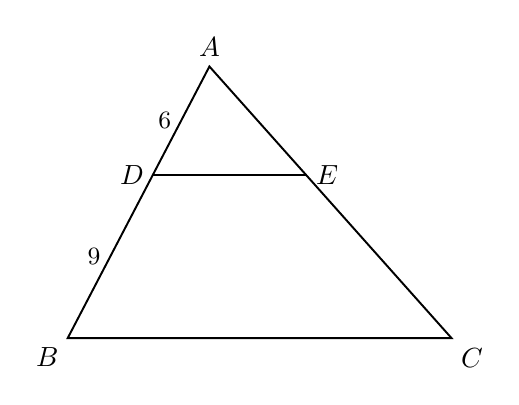
\begin{tikzpicture}[scale=0.75,>=latex]
\coordinate (B) at (0,0); \coordinate (C) at (6.5,0); \coordinate (A) at (2.4,4.6);
\coordinate (D) at ($(A)!0.4!(B)$); \coordinate (E) at ($(A)!0.4!(C)$);
\draw[line width=0.7pt] (A)--(B)--(C)--cycle;
\draw[line width=0.7pt] (D)--(E);
\node[above] at (A) {$A$}; \node[below left] at (B) {$B$}; \node[below right] at (C) {$C$};
\node[left] at (D) {$D$}; \node[right] at (E) {$E$};
\node[left,font=\small] at ($(A)!0.2!(B)$) {6};
\node[left,font=\small] at ($(D)!0.5!(B)$) {9};
\end{tikzpicture}}\gridbox
\vfill

\noindent\pnum{22} In the equation below, $k$ is a constant.\dsp{$\dfrac{x-1}{x-k}=\dfrac{x+3}{x-2}$}What is the sum of all values of $k$ for which the equation has no solution?\par\vspace{2.2mm}
\hspace*{7mm}(A)\ $3$\\[1.8mm]
\hspace*{7mm}(B)\ $6$\\[1.8mm]
\hspace*{7mm}(C)\ $8$\\[1.8mm]
\hspace*{7mm}(D)\ $9$
\vfill}}
\end{textblock*}
\clearpage

\end{document}
